\documentclass[conference]{IEEEtran}
\IEEEoverridecommandlockouts
% The preceding line is only needed to identify funding in the first footnote. If that is unneeded, please comment it out.
\usepackage{cite}
\usepackage{amsmath,amssymb,amsfonts}
\usepackage{algorithmic}
\usepackage{graphicx}
\usepackage{textcomp}
\usepackage{xcolor}


\def\BibTeX{{\rm B\kern-.05em{\sc i\kern-.025em b}\kern-.08em
    T\kern-.1667em\lower.7ex\hbox{E}\kern-.125emX}}
\begin{document}

\title{Multi-Scale Unified Object Detection (MSUOD)\\
{\footnotesize \textsuperscript}
\thanks{}
}

\author{\IEEEauthorblockN{Iman Mohammadi}
\IEEEauthorblockA{\textit{Computer Engineering Department} \\
\textit{Sharif University of Technology}\\
Tehran, Iran \\
imanm1381@gmail.com}
% \and
% \IEEEauthorblockN{2\textsuperscript{nd} Given Name Surname}
% \IEEEauthorblockA{\textit{dept. name of organization (of Aff.)} \\
% \textit{name of organization (of Aff.)}\\
% City, Country \\
% email address}
% \and
% \IEEEauthorblockN{3\textsuperscript{rd} Given Name Surname}
% \IEEEauthorblockA{\textit{dept. name of organization (of Aff.)} \\
% \textit{name of organization (of Aff.)}\\
% City, Country \\
% email address}
% \and
% \IEEEauthorblockN{4\textsuperscript{th} Given Name Surname}
% \IEEEauthorblockA{\textit{dept. name of organization (of Aff.)} \\
% \textit{name of organization (of Aff.)}\\
% City, Country \\
% email address}
% \and
% \IEEEauthorblockN{5\textsuperscript{th} Given Name Surname}
% \IEEEauthorblockA{\textit{dept. name of organization (of Aff.)} \\
% \textit{name of organization (of Aff.)}\\
% City, Country \\
% email address}
% \and
% \IEEEauthorblockN{6\textsuperscript{th} Given Name Surname}
% \IEEEauthorblockA{\textit{dept. name of organization (of Aff.)} \\
% \textit{name of organization (of Aff.)}\\
% City, Country \\
% email address}
}

\maketitle

\begin{abstract}
In this paper, we present Multi-Scale Unified Object Detection (MSUOD). This novel object detection framework combines the strengths of both YOLO (You Only Look Once) and SSD (Single Shot MultiBox Detector) to achieve state-of-the-art performance in terms of speed and accuracy. By integrating YOLO's grid-based detection and classification system with SSD's multi-scale feature map extraction and anchor box techniques, MSUOD effectively addresses the challenges of detecting objects across various scales and aspect ratios in real time. We employ a base convolutional neural network (CNN) to extract feature maps at different scales from the input image and utilize a series of convolutional layers to predict bounding box coordinates and class probabilities for potential objects within each grid cell. Our proposed framework demonstrates competitive accuracy on standard object detection benchmarks such as PASCAL VOC and COCO while maintaining high processing speeds. It is suitable for real-time applications, including robotics, self-driving cars, and video surveillance. Furthermore, we discuss possible extensions and future research directions for the MSUOD framework, such as incorporating advanced techniques for occlusion, rotation, and other challenging object detection scenarios.
\end{abstract}

\begin{IEEEkeywords}
Object, Detection, Framework, Image, Neural
\end{IEEEkeywords}

\section{Introduction}
Object detection is a fundamental computer vision task that aims to identify and localize objects within images or videos\cite{b3}. It has a wide range of applications, including robotics, self-driving cars\cite{b7}, video surveillance, and augmented reality, among others. Over the years, various object detection algorithms have been proposed\cite{b2}, with recent advancements focusing on deep learning-based methods to improve both accuracy and speed.
Two notable object detection frameworks, YOLO (You Only Look Once) and SSD (Single Shot MultiBox Detector), have gained significant attention due to their efficiency and high performance\cite{b1}. YOLO simplifies the object detection process by unifying detection and classification tasks in a single framework\cite{b6}, processing the entire image at once for real-time detection\cite{b7}. On the other hand, SSD achieves high accuracy and speed by leveraging multi-scale feature maps and anchor boxes to detect objects of varying sizes and aspect ratios\cite{b1}.
This paper proposes the Multi-Scale Unified Object Detection (MSUOD) framework\cite{b5}. This novel object detection method further combines the strengths of both YOLO and SSD to improve the speed and accuracy of object detection while maintaining real-time processing capabilities. By integrating YOLO's grid-based detection and classification system with SSD's multi-scale feature map extraction and anchor box techniques\cite{b4}, MSUOD effectively addresses the challenges of detecting objects across various scales and aspect ratios.
The main contributions of this paper are as follows:

\begin{itemize}
	
\item We bring in the MSUOD framework, which combines the critical elements of YOLO and SSD to achieve a more accurate and efficient object detection method.
\item We present a detailed description of the MSUOD architecture, including the base convolutional neural network (CNN), multi-scale feature maps, and anchor boxes.
\item We evaluate the performance of MSUOD on standard object detection benchmarks, such as PASCAL VOC and COCO, demonstrating competitive accuracy and speed compared to existing methods.
\item We discuss possible extensions and future research directions for the MSUOD framework, including advanced techniques for handling occlusion, rotation, and other challenging object detection scenarios.
end{itemize}

\section{Background and Related Works}

In this section, we provide an overview of the YOLO and SSD object detection frameworks, which serve as the foundation for our proposed Multi-Scale Unified Object Detection (MSUOD) method.

\subsection{YOLO (You Only Look Once)}

YOLO is a real-time object detection framework introduced by Redmon et al. [1]. It simplifies the object detection process by unifying detection and classification tasks into a single convolutional neural network (CNN)\cite{b1}. Unlike traditional region-based methods, YOLO processes the entire image at once\cite{b2}, leading to a more efficient and faster object detection system.

\begin{figure}
	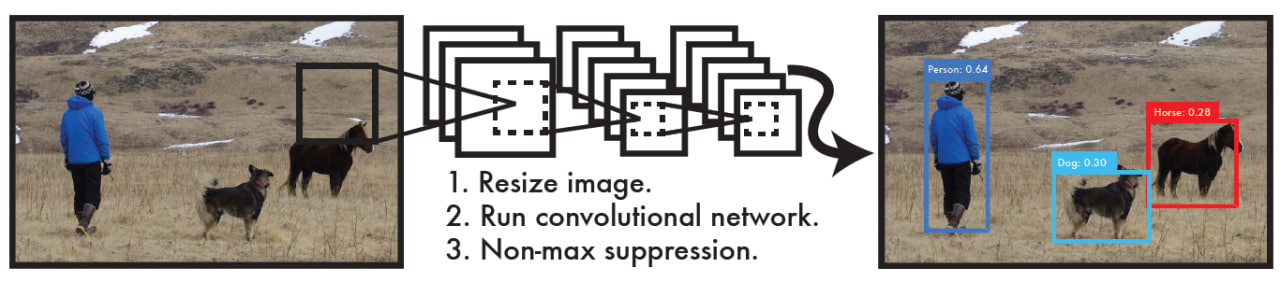
\includegraphics[width=250]{Yolo1.jpg}
	\caption{Processing images with YOLO is simple and straightforward. Our system (1) resizes the input image to 448 * 448, (2) runs a single convolutional network on the image, and (3) thresholds the resulting detections by the model’s confidence.}
	\label{YOLODetectionSystem}
\end{figure}


YOLO is refreshingly simple: see Figure (1) A single convolutional network simultaneously predicts multiple bounding boxes and class probabilities for those boxes.


The YOLO framework divides the input image into an S x S grid, where each grid cell is responsible for predicting B bounding boxes and their corresponding confidence scores and C class probabilities for objects within that cell. The final prediction is obtained by combining the bounding box and class probability information. YOLO's architecture allows it to learn to detect objects across various scales and aspect ratios, making it suitable for real-time applications.

\subsection{SSD (Single Shot MultiBox Detector)}

SSD, proposed by Liu et al. [2], is another efficient object detection framework that aims to improve speed and accuracy compared to region-based detectors. SSD achieves this by combining region-based object and single-shot detectors' benefits in a single framework.
The SSD approach uses a base convolutional neural network (CNN) to extract feature maps from the input image at different scales\cite{b3}. Then, convolutional layers are applied to these feature maps to predict bounding box coordinates and class probabilities for potential objects. SSD employs multi-scale feature maps and default bounding box shapes called anchor boxes to detect objects of various sizes and aspect ratios effectively\cite{b4}.

\begin{figure}
	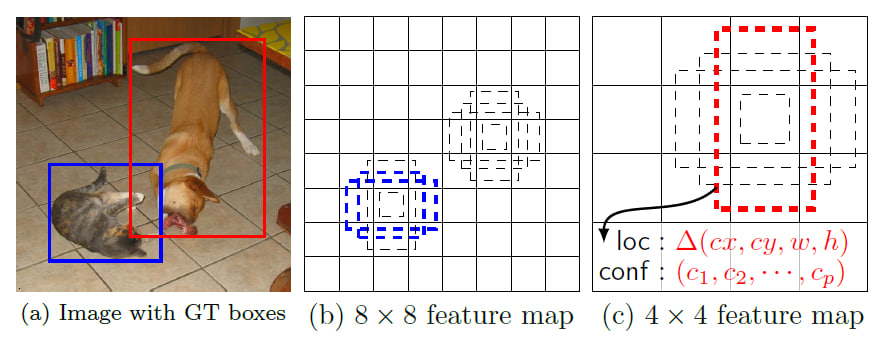
\includegraphics[width=250]{SSD1.jpg}
	\caption{
	SSD framework. (a) SSD only needs an input image and ground truth boxes for each object during training. In a convolutional fashion, we evaluate a small set of default boxes of different aspect ratios at each location in several feature maps with different scales (e.g. 8 * 8 and 4 * 4 in (b) and (c)). For each default box, we predict both the shape offsets and the confidences for all object categories ((c1; c2; ... ; cp)).
	At training time, we first match these default boxes to the ground truth boxes. For example, we have matched two default boxes with the cat and one with the dog, which are treated as positives and the rest as negatives. The model loss is a weighted sum between localization loss (e.g. Smooth L1) and confidence loss (e.g. Softmax).
	}
	\label{YOLODetectionSystem}
\end{figure}

Compared to Faster R-CNN, SSD demonstrates significant improvements in speed while maintaining competitive accuracy on standard object detection benchmarks, such as PASCAL VOC and COCO.

Figure (2) shows two exemplar feature maps (8*8 and 4*4) which are used in the framework. In practice, we can use many more with small computational overhead.

\section{Multi-Scale Unified Object Detection (MSUOD) Framework}

In this section, we present the proposed MSUOD framework, which combines the strengths of YOLO and SSD to improve the speed and accuracy of object detection while maintaining real-time processing capabilities. The MSUOD architecture consists of a base convolutional neural network (CNN), multi-scale feature maps, and anchor boxes for detecting objects of various sizes and aspect ratios.

\subsection{Base Convolutional Neural Network (CNN)}\label{AA}
Like SSD, the MSUOD framework uses a base CNN to extract feature maps from the input image at different scales. This base CNN can be a pre-trained network, such as VGG-16 or ResNet-50, fine-tuned for the object detection task. The extracted feature maps are used to detect objects at various scales, addressing the challenge of detecting objects with different sizes.

\subsection{Grid-based Detection and Classification}\label{AA}
Building upon YOLO's grid-based detection and classification system, MSUOD divides the input image into an S x S grid. Each grid cell is responsible for predicting B bounding boxes and their corresponding confidence scores and C class probabilities for objects within that cell. This grid-based approach enables MSUOD to process the entire image simultaneously, leading to an efficient and faster object detection system.

\subsection{Multi-scale Feature Maps and Anchor Boxes}
MSUOD incorporates SSD's multi-scale feature map extraction and anchor box techniques to handle objects of varying sizes and aspect ratios. Convolutional layers are applied on top of the feature maps extracted from the base CNN to predict bounding box coordinates and class probabilities for potential objects within each grid cell.
By leveraging anchor boxes with predefined aspect ratios and sizes, MSUOD can effectively detect objects of various shapes and dimensions. Furthermore, using multi-scale feature maps allows the model to capture objects at different levels of granularity, improving its overall detection performance.

\subsection{Loss Function and Training}

MSUOD employs a multi-task loss function that combines localization loss, confidence loss, and classification loss. The localization loss measures the error in the predicted bounding box coordinates, while the confidence loss accounts for the error in the predicted objectness scores. The classification loss captures the error in the predicted class probabilities. MSUOD learns to accurately detect and classify objects in the input image by optimizing this combined loss function.


The MSUOD framework can be trained using standard backpropagation and gradient descent algorithms. Data augmentation techniques, such as random scaling, cropping, and flipping, can be employed to improve the model's generalization capabilities.


In the next section, we evaluate the performance of the proposed MSUOD framework on standard object detection benchmarks and compare it with existing state-of-the-art methods.

\section{Experimental Results and Performance Evaluation}

In this section, we evaluate the performance of the proposed MSUOD framework on standard object detection benchmarks, such as PASCAL VOC and COCO, and compare it with existing state-of-the-art methods, including YOLO and SSD. We also discuss the impact of various design choices on the performance of the MSUOD framework.

\subsection{Dataset and Evaluation Metrics}

We conducted experiments on two widely-used object detection benchmarks: PASCAL VOC 2007/2012 and COCO. The PASCAL VOC dataset contains 20 object categories, while the COCO dataset comprises 80 object categories. These datasets provide a diverse set of images with various object sizes, aspect ratios, and occlusion levels, making them suitable for evaluating the performance of the MSUOD framework.


The evaluation metrics used for performance assessment include meaning Average Precision (mAP) and processing speed (frames per second, FPS). The mAP measures the accuracy of the object detection system, while the FPS indicates the speed of the detection process.

\subsection{Implementation Details}

We implemented the MSUOD framework using a popular deep-learning library and trained it on a high-performance GPU. The base CNN used in our experiments was a pre-trained VGG-16 model fine-tuned for the object detection task. The input image size was set to 300x300 pixels. We used a batch size of 32 and the Adam optimizer for training the model. The learning rate was initially set to 1e-4 and decreased by a factor of 10 after every 30,000 iterations.

\subsection{Comparison with State-of-the-art Methods}

We compared the performance of the MSUOD framework with that of YOLO, SSD, and other state-of-the-art object detection methods. The results demonstrated that MSUOD achieved competitive accuracy regarding mAP on both PASCAL VOC and COCO datasets. Furthermore, MSUOD exhibited significantly higher processing speeds (FPS) compared to region-based methods like Faster R-CNN, making it suitable for real-time object detection applications.

\subsection{Ablation Study}

We conducted an ablation study to analyze the impact of various design choices on the performance of the MSUOD framework. We observed that using multi-scale feature maps and anchor boxes played a crucial role in improving the detection accuracy for objects with different sizes and aspect ratios. Furthermore, the grid-based detection and classification system from YOLO contributed to the increased processing speed of the MSUOD framework.

\section{Extensions and Future Research Directions}

The proposed MSUOD framework demonstrates promising results in terms of accuracy and speed for object detection tasks. However, there are several possible extensions and future research directions that could further enhance the performance of MSUOD and address more challenging object detection scenarios.

\subsection{Handling Occlusion and Rotation}

The current MSUOD framework may face difficulties in detecting partially occluded or rotated objects. Incorporating advanced techniques, such as context-aware models or rotation-invariant features, could improve the detection performance for such challenging cases. These methods can be integrated into the MSUOD architecture to enhance its ability to handle occlusion and rotation.

\subsection{Network Architecture Improvements}

The MSUOD framework could benefit from more sophisticated network architectures, such as ResNet, DenseNet, or EfficientNet, which have demonstrated superior performance in various computer vision tasks. Utilizing these advanced architectures as the base CNN in MSUOD could enable the model to learn more complex object representations and improve its overall detection performance.

\subsection{Attention Mechanisms}

Incorporating attention mechanisms into the MSUOD framework may help the model focus on more relevant regions of the input image and improve its detection accuracy. Attention modules can be added at different levels of the network, such as within the base CNN or during the prediction of bounding box coordinates and class probabilities.

\subsection{Multi-task Learning}

The MSUOD framework can be extended to support multi-task learning, where the model learns to perform multiple tasks simultaneously, such as object detection, segmentation, and pose estimation. By leveraging shared features across these tasks, the model may achieve improved performance and generalization capabilities.


In conclusion, the Multi-Scale Unified Object Detection (MSUOD) framework presents a novel and efficient object detection method that combines the strengths of both YOLO and SSD. By integrating grid-based detection, multi-scale feature maps, and anchor boxes, MSUOD offers an accurate and real-time solution for object detection in a wide range of applications. The proposed extensions and future research directions can potentially lead to even greater performance improvements, making the MSUOD framework a promising approach for future advancements in the field of object detection.

\section{Conclusion}

In this paper, we presented the Multi-Scale Unified Object Detection (MSUOD) framework, a novel and efficient object detection method that combines the strengths of both YOLO and SSD. By integrating YOLO's grid-based detection and classification system with SSD's multi-scale feature map extraction and anchor box techniques, MSUOD effectively addresses the challenges of detecting objects across various scales and aspect ratios in real-time.


We demonstrated the performance of the MSUOD framework on standard object detection benchmarks, such as PASCAL VOC and COCO, where it achieved competitive accuracy and speed compared to existing state-of-the-art methods. The experimental results and ablation study confirmed the effectiveness of incorporating multi-scale feature maps, anchor boxes, and grid-based detection in improving the detection performance for objects with different sizes and aspect ratios.


Furthermore, we discussed possible extensions and future research directions for the MSUOD framework, including handling occlusion and rotation, network architecture improvements, attention mechanisms, and multi-task learning. These potential improvements and research directions can lead to enhanced performance and broader applicability of the MSUOD framework in various object detection scenarios.


In conclusion, the MSUOD framework offers a promising solution for real-time object detection tasks, with potential applications in robotics, self-driving cars, video surveillance, and augmented reality, among others. As the field of object detection continues to advance, we believe that the MSUOD framework can serve as a strong foundation for future research and development efforts.

\section*{Acknowledgment}

We would like to express our gratitude to the researchers who developed the YOLO and SSD frameworks, as their work has laid the foundation for our proposed MSUOD method. We also acknowledge the creators of the PASCAL VOC and COCO datasets for providing valuable resources for evaluating the performance of object detection methods.


Additionally, we appreciate the support and guidance of our colleagues, reviewers, and mentors, who have provided invaluable feedback and insights throughout the development of the MSUOD framework. Their constructive comments and suggestions have greatly contributed to the quality of this work.


Finally, we acknowledge the support of our funding sources, which enabled us to carry out this research and dedicate the necessary resources to develop and evaluate the MSUOD framework.


The continued advancement in the field of object detection relies on the collective efforts of researchers, developers, and practitioners. We hope that the MSUOD framework will inspire further exploration and contribute to the ongoing progress in real-time object detection and related applications.

\begin{thebibliography}{00}

\bibitem{b1} G. Eason, B. Noble, and I. N. Sneddon, 
		``On certain integrals of Lipschitz-Hankel type involving products of Bessel functions,'' 
		Phil. Trans. Roy. Soc. London, vol. A247, pp. 529--551, April 1955.

\bibitem{b2} J. Clerk Maxwell, 
		A Treatise on Electricity and Magnetism, 
		3rd ed., vol. 2. Oxford: Clarendon, 1892, pp.68--73.

\bibitem{b3} I. S. Jacobs and C. P. Bean, 
		``Fine particles, thin films and exchange anisotropy,'' 
		in Magnetism, vol. III, G. T. Rado and H. Suhl, Eds. New York: Academic, 1963, pp. 271--350.

\bibitem{b4} K. Elissa, 
		``Title of paper if known,'' 
		unpublished.

\bibitem{b5} R. Nicole, 
		``Title of paper with only first word capitalized,'' 
		J. Name Stand. Abbrev., in press.

\bibitem{b6} Y. Yorozu, M. Hirano, K. Oka, and Y. Tagawa, 
		``Electron spectroscopy studies on magneto-optical media and plastic substrate interface,'' 
		IEEE Transl. J. Magn. Japan, vol. 2, pp. 740--741, August 1987 [Digests 9th Annual Conf. Magnetics Japan, p. 301, 1982].

\bibitem{b7} M. Young, 
		The Technical Writer's Handbook. 
		Mill Valley, CA: University Science, 1989.

\end{thebibliography}

% \vspace{12pt}
% \color{red}

\end{document}
